% Chapter 3

\chapter{Marco metodológico}

\label{Chapter3}

%---------------------------------------------------

\section{Estado del arte}

El uso de inteligencia artificial en el sector agroalimentario ha crecido significativamente durante la última década, especialmente en áreas como clasificación de frutas, detección de defectos, estimación de madurez y predicción de vida útil. Este avance ha sido impulsado tanto por el desarrollo de modelos de aprendizaje profundo como por la disponibilidad de sensores ópticos más accesibles. Sin embargo, en cultivos específicos como el dátil Medjool, la aplicación práctica de estas tecnologías sigue siendo limitada.\\

\parencite{kamilaris_deep_2018} realizaron una revisión temprana sobre el uso de redes neuronales y visión por computadora en agricultura, estableciendo las bases para su uso en tareas de clasificación de cultivos y análisis de calidad. Estudios como el de \parencite{garcia_vazquez_scientometric_2021, upadhyay_artificial_2025} han documentado el crecimiento de estas aplicaciones, enfatizando la necesidad de enfoques más integrales y adaptados a entornos reales.\\

En los últimos años, la disponibilidad de \textit{datasets} públicos relacionados con la evaluación de dátiles y otros frutos ha crecido de forma considerable. Estos \textit{datasets}, que pueden incluir imágenes etiquetadas por madurez, espectros ópticos o atributos físico-químicos, han permitido el desarrollo y comparación de modelos de clasificación, segmentación y regresión en distintas condiciones experimentales. Algunos de estos recursos se centran en variedades específicas como Medjool o Mejhoul, y otros en condiciones agrícolas más generales. La revisión de estos conjuntos de datos es útil no solo para complementar el entrenamiento de modelos, sino también como referencia para el diseño de nuevas estrategias de adquisición de datos. En la Tabla \ref{tab:datasets} se presenta una síntesis de los \textit{datasets} más relevantes identificados durante la revisión bibliográfica.\\

En el caso específico de frutas, múltiples autores han demostrado la eficacia de modelos convolucionales para clasificar variedades, predecir estado de madurez o detectar enfermedades superficiales \parencite{rybacki_convolutional_2024, gill_fruit_2023, almomen_date_2023}. Estos algoritmos aprenden directamente de las imágenes y permiten eliminar pasos de preprocesamiento complejos, siempre que cuenten con \textit{datasets} balanceados y representativos.\\

En paralelo, la espectroscopía \textit{NIR} ha ganado espacio como técnica no destructiva para estimar características internas de los frutos, como contenido de humedad o azúcares. Estudios como los de \parencite{yuan_determination_2025, wang_improving_2025, chen_prediction_2024} muestran cómo la combinación de \textit{NIR} con modelos de redes neuronales mejora considerablemente la precisión en predicciones fisicoquímicas.\\

Una tendencia emergente es la integración de distintos tipos de datos en modelos multimodales, como imágenes \textit{RGB}, espectros \textit{NIR} y parámetros colorimétricos, lo que ha demostrado ser más robusto frente a variabilidad ambiental y condiciones no controladas \parencite{said_smartripen_2025, passos_deep_2023}. Estos enfoques también permiten predecir variables difíciles de observar a simple vista, como la presencia de hongos o la pérdida de firmeza.\\

Aunque estas técnicas han sido aplicadas exitosamente en frutas como manzana, mango, papaya y jujube, su implementación en \textit{Phoenix dactylifera L.}, y en particular en el dátil Medjool cultivado en México, aún está poco documentada. Algunos trabajos recientes han explorado la clasificación superficial mediante \textit{CNNs} \parencite{perez-perez_evaluation_2021}, pero la evaluación de características internas sigue siendo un campo abierto, especialmente desde una perspectiva de bajo costo y accesibilidad técnica.\\

En línea con la necesidad de hacer los modelos de aprendizaje profundo más transparentes y confiables, ha surgido un campo conocido como inteligencia artificial explicable (\textit{XAI}). Técnicas como \textit{Grad-CAM}, utilizada para visualizar regiones activadas en \textit{CNNs} aplicadas a imágenes, o \textit{SHAP}, aplicada a modelos de regresión o clasificación con datos espectrales, permiten interpretar cómo y por qué un modelo toma determinadas decisiones. Estas herramientas no solo ayudan a mejorar la confianza en el sistema, sino que también permiten detectar posibles sesgos o errores estructurales en el entrenamiento \parencite{russel_wavelet_2024, gupta_fruveg-net_2024}.\\

Por lo tanto, existe un área de oportunidad clara para aplicar y adaptar estos avances al caso del dátil Medjool, desarrollando soluciones tecnológicamente viables para productores de la región que necesitan herramientas confiables, no destructivas y económicas.

\newpage

%---------------------------------------------------

\section{Metodología}

La metodología de este estudio está basada en una adaptación del modelo \textit{CRISP-DM} (\textit{Cross-Industry Standard Process for Data Mining}), una de las guías más reconocidas y utilizadas en ciencia de datos aplicada. En la Figura \ref{fig:componentes} se muestra como \textit{CRISP-DM} organiza el proceso analítico en seis fases cíclicas: comprensión del negocio, comprensión de los datos, preparación de los datos, modelado, evaluación e implementación. Su carácter flexible e iterativo permite adaptarse a distintas áreas del conocimiento, incluyendo dominios con datos no estructurados, como es el caso de los sistemas agrícolas \parencite{shimaoka_evolution_2024, saltz_crisp-dm_2021}. En este trabajo, la metodología se ha modificado para ajustarse al contexto particular de la evaluación de calidad postcosecha del dátil Medjool, integrando técnicas de aprendizaje profundo, sensores ópticos y validación experimental en condiciones reales.

\begin{figure}[th]
\centering
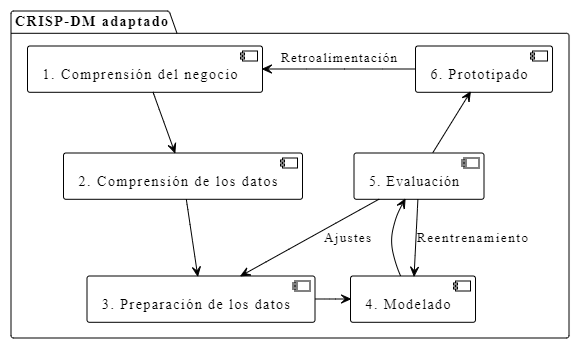
\includegraphics[scale=0.75]{Figures/componentes.png}
\decoRule
\caption{Diagrama de componentes \textit{CRISP-DM} ajustado.}
\label{fig:componentes}
\end{figure}

\subsection{Fase 1: Comprensión del dominio agrícola y científico}

La primera fase tiene como objetivo comprender a profundidad el contexto en el que se desarrollará el estudio, tanto desde la práctica agrícola como desde la perspectiva científica. Desde el ámbito productivo, se analizará cómo se realiza actualmente la evaluación de calidad postcosecha del dátil Medjool en el Valle de Mexicali. Mediante entrevistas, observación directa y colaboración con productores locales, se documentarán las prácticas manuales utilizadas, los criterios empíricos aplicados en la selección de frutos y las variables que los operarios consideran más relevantes para determinar la calidad comercial.\\

En paralelo, se llevará a cabo una revisión de la literatura científica especializada sobre evaluación no destructiva de calidad en frutos, con especial atención a trabajos que hayan implementado modelos predictivos o clasificadores utilizando variables físico-químicas, espectrales o colorimétricas. Aunque muchos de estos estudios se centran en otros cultivos, sus metodologías, variables utilizadas y resultados obtenidos servirán como base comparativa para identificar parámetros clave y justificar su inclusión en el enfoque propuesto.\\

Este doble enfoque, productivo y científico, permitirá fundamentar con solidez las decisiones posteriores del estudio, garantizando que el enfoque multimodal desarrollado sea relevante, contextualizado y con potencial de generalización.

\subsection{Fase 2: Comprensión y caracterización de los datos}

Esta fase se enfoca en el análisis exploratorio de las muestras que conformarán la base empírica del estudio. Se recolectarán dátiles Medjool representativos de distintas etapas de madurez y condiciones postcosecha, incluyendo tanto ejemplares en óptimas condiciones como otros con signos de sobremadurez o posibles defectos internos. Esta diversidad permitirá evaluar la capacidad del enfoque multimodal para capturar gradaciones en la calidad del fruto que no siempre son evidentes de forma visual o superficial.\\

Antes de cualquier intervención destructiva, cada fruto será sometido a la adquisición de imágenes \textit{RGB} en condiciones controladas, junto con la medición de espectros en el rango infrarrojo cercano y la estimación colorimétrica en el espacio CIELab. Estos datos ópticos se obtendrán de forma no invasiva, asegurando que el estado del fruto se registre de manera íntegra para ser correlacionado posteriormente con las variables físico-químicas de referencia. Esta precaución es esencial, ya que algunas de las pruebas subsiguientes, como la evaluación interna o la determinación del contenido de humedad, implican la destrucción de la muestra.\\

Cada muestra será sometida a una serie de mediciones físico-químicas que funcionarán como etiquetas de referencia para el posterior entrenamiento y validación de modelos. El contenido de humedad será determinado, idealmente, mediante el método de secado en horno con peso constante, que constituye el estándar de referencia por su precisión. La firmeza será evaluada mediante instrumentos como texturómetros o penetrómetros digitales, que permiten cuantificar la resistencia mecánica del tejido en unidades estandarizadas. Por su parte, el estado interno del fruto se determinará mediante inspección visual tras un corte, permitiendo registrar la presencia de defectos como fermentación interna, colapso del mesocarpio o desarrollo de hongos. La Tabla \ref{tab:metodos} resume las variables a medir y los métodos de adquisición propuestos.\\

\begin{table}[h]
\footnotesize
\centering
\begin{tabular}{|p{5cm}|p{2.5cm}|p{3cm}|p{2.5cm}|}
\hline
\textbf{Título del artículo} & \textbf{Variedad(es)} & \textbf{Tipo de datos} & \textbf{Acceso al \textit{dataset}} \\
\hline

\textit{Dataset for localization and classification of Medjool dates in digital images} \newline \parencite{perez-perez_dataset_2021} & Medjool & Imágenes \textit{RGB} con anotaciones & \href{https://data.mendeley.com/datasets/872xk9npmz/1}{Mendeley Data} \\

\hline

\textit{Date fruit dataset for intelligent harvesting} \newline \parencite{altaheri_date_2019} & Barhi, Sullaj, Meneifi, Khalas, Naboot Saif & \textit{RGB} en distintas etapas de madurez & \href{https://ieee-dataport.org/open-access/date-fruit-dataset-automated-harvesting-and-visual-yield-estimation}{IEEE DataPort} \\

\hline

\textit{Date fruit detection dataset for automatic harvesting} \newline \parencite{zarouit_date_2024} & Variadas (4) & \textit{RGB}, imágenes y videos para detección automática & \href{https://zenodo.org/records/10143465}{Zenodo} \\

\hline

\textit{Comprehensive characterization of date palm fruit ‘Mejhoul’ using image analysis} \newline \parencite{noutfia_comprehensive_2022} & Mejhoul & Imágenes \textit{RGB}, colorimetría y texturas & Acceso bajo petición \\

\hline

\end{tabular}
\caption{\textit{Datasets} públicos de estudios sobre dátiles.}
\label{tab:datasets}
\end{table}

Complementariamente, se llevará a cabo una búsqueda y análisis de \textit{datasets} públicos que hayan sido utilizados en estudios previos sobre evaluación de dátiles u otros frutos similares, algunos se muestran en la Tabla \ref{tab:datasets}. Se revisarán bases de datos abiertos disponibles en artículos científicos recientes, con énfasis en aquellos que incluyen imágenes \textit{RGB}, espectros \textit{NIR}, parámetros físico-químicos o etiquetas de clasificación. Estos recursos podrán ser aprovechados para extender el análisis, validar modelos en contextos externos o comparar el desempeño del enfoque desarrollado con resultados publicados.\\

Este conjunto de acciones permitirá construir una base de datos robusta y representativa, que combine observaciones empíricas locales con referencias científicas reconocidas, y que sirva de soporte para el diseño y evaluación de modelos predictivos no destructivos en fases posteriores.

\begin{table}[h]
\centering
\footnotesize
\begin{tabular}{|p{4.5cm}|p{9cm}|}
\hline
\textbf{Variable} & \textbf{Método de medición} \\
\hline

\textbf{Datos ópticos} &
Cámara profesional para adquisición de imágenes \textit{RGB}. Espectrómetro para obtención de información en las bandas \textit{NIR}. \\
\hline

\textbf{Firmeza (N)} &
Penetrómetro digital o texturómetro. Presión o fuerza aplicada al fruto para determinar su resistencia mecánica. \\
\hline

\textbf{Estado interno (defectos, hongos)} &
Inspección visual tras corte transversal. Validación cualitativa de condiciones internas no visibles externamente. \\
\hline

\textbf{Contenido de humedad (\%)} &
Secado en horno con peso constante:
\[
\text{Humedad (\%)} = \frac{P_{\text{fresco}} - P_{\text{seco}}}{P_{\text{fresco}}} \times 100
\]
\\
\hline

\end{tabular}
\caption{Variables fisicoquímicas y métodos de medición.}
\label{tab:metodos}
\end{table}

\subsection{Fase 3: Preparación de los datos}

Una vez obtenidas las muestras, se realizará la organización y procesamiento de los datos recolectados para su análisis. En esta fase se integrará la información proveniente de múltiples fuentes, incluyendo las imágenes \textit{RGB} de los frutos, los espectros en el rango infrarrojo cercano (\textit{NIR}), los parámetros colorimétricos extraídos (L*, a*, b*), así como las mediciones físico-químicas de referencia obtenidas en laboratorio o por inspección directa. La Figura \ref{fig:adquisicion} en el \nameref{AnexoA} muestra una versión simplificada del flujo a seguir.\\

Cada unidad de análisis (es decir, cada fruto individual) será representada por un conjunto estructurado de datos que combinará estas distintas modalidades. Para ello, se establecerán identificadores únicos por muestra que permitan sincronizar correctamente los distintos tipos de entrada y sus etiquetas. El procesamiento de datos incluirá la limpieza de registros incompletos, la eliminación de ruido espectral, y la normalización de valores numéricos a través de métodos como Savitzky-Golay para espectros y estandarización Z-score para otras variables.\\

El resultado de esta fase será un conjunto de datos multimodal, limpio y organizado, adecuado para su uso en tareas supervisadas de clasificación y regresión. Este \textit{dataset} representará tanto las características ópticas del fruto como su estado físico-químico confirmado, permitiendo entrenar modelos que busquen inferir calidad postcosecha de manera no destructiva. Además, la estructura de los datos permitirá comparar el desempeño de modelos unimodales (basados en un solo tipo de entrada) frente a modelos multimodales, como parte del análisis posterior.

\subsection{Fase 4: Modelado}

En esta fase se diseñará y entrenará un conjunto de modelos de aprendizaje supervisado con el objetivo de predecir variables críticas de calidad postcosecha del dátil Medjool a partir de los datos ópticos multimodales obtenidos. Los modelos desarrollados abarcarán tanto enfoques unimodales (basados en un solo tipo de entrada como espectros \textit{NIR} o imágenes \textit{RGB}) como enfoques multimodales que integren múltiples tipos de datos de manera simultánea (\textit{RGB} + \textit{NIR}).\\

Para las tareas de clasificación, como la detección de defectos internos o categorización de madurez, se entrenarán modelos de \textit{CNNs} aplicadas a imágenes, y modelos multicapas densamente conectados (\textit{MLP}) aplicados a espectros. En las tareas de regresión, especialmente en la predicción del contenido de humedad, se evaluarán tanto modelos de redes neuronales como métodos clásicos de regresión multivariada como \textit{PLSR} (\textit{Partial Least Squares Regression}), que servirán como línea base para la comparación.\\

Los modelos serán ajustados mediante procesos de validación cruzada y búsqueda de hiperparámetros, utilizando criterios como la raíz del error cuadrático medio (\textit{RMSE}), el coeficiente de determinación (\textit{$R^2$}) en regresión, y métricas como precisión, sensibilidad, especificidad y \textit{F1-score} en clasificación. Además, se explorarán diferentes estrategias de fusión de datos (temprana, intermedia o tardía) para evaluar cómo la integración de modalidades afecta el desempeño predictivo.\\

Este proceso no solo permitirá construir modelos con potencial predictivo, sino que también generará evidencia sobre qué tipo de datos y combinaciones ofrecen mayor valor informativo. Así, se podrá comparar directamente la eficacia de modelos basados únicamente en imágenes, en espectros o en datos colorimétricos, frente a aquellos que aprovechan la complementación de todos ellos.

\subsection{Fase 5: Evaluación}

La fase de evaluación tiene como objetivo valorar el desempeño del enfoque multimodal propuesto desde múltiples dimensiones: precisión predictiva, robustez estadística, interpretabilidad del modelo y aplicabilidad en condiciones reales. Esta etapa es fundamental para determinar si los modelos desarrollados pueden generalizarse a nuevas muestras, conservar su rendimiento ante condiciones no controladas y ofrecer resultados útiles para la toma de decisiones postcosecha.\\

Además del análisis numérico, se integrarán herramientas de \textit{XAI} que permitirán interpretar el comportamiento interno de los modelos. Estas técnicas ofrecen una forma de visualizar qué variables influyen más en las predicciones, brindando transparencia a los procesos de inferencia. Se empleará \textit{Grad-CAM} para analizar activaciones en modelos basados en imágenes, y \textit{SHAP} para modelos que utilicen entradas espectrales o numéricas \parencite{lundberg_unified_2017}. Esta combinación permitirá contrastar las predicciones con el conocimiento experto y detectar posibles sesgos, patrones significativos o errores sistemáticos.\\

Para los métodos propuestos, se considerarán las siguientes métricas de evaluación:
\begin{itemize}
    \item \textbf{Regresión:} \textit{RMSE}, \textit{MAE}, \textit{R2}.
    \item \textbf{Clasificación:} Precisión, sensibilidad, \textit{F1-score}, \textit{AUC-ROC}.
\end{itemize}

Estas métricas permitirán evaluar tanto la precisión de los modelos como su capacidad para generalizar a nuevas muestras y su interpretabilidad, lo que es crucial para la confianza en aplicaciones prácticas. En el \nameref{AnexoB} se habla de forma más detallada sobre cada una de estas métricas y su aplicación en el contexto del presente estudio.

\subsection{Fase 6: Prototipado}

La última fase del proceso metodológico consistirá en el desarrollo de un prototipo funcional que permita validar, de forma práctica y exploratoria, la aplicabilidad del enfoque multimodal en condiciones operativas. Este prototipo no se plantea como un producto final, sino como una herramienta experimental para poner a prueba el flujo de adquisición, análisis y predicción en entornos reales, tales como empacadoras o laboratorios agrícolas.\\

El prototipo consistirá en un conjunto de componentes conectados que integren, por un lado, el proceso de adquisición de datos ópticos (\textit{RGB}, \textit{NIR}, CIELab) y, por otro, la inferencia de variables de calidad mediante los modelos entrenados. La arquitectura tecnológica se mantendrá abierta, con la posibilidad de ejecutar los modelos en entornos de prueba como Jupyter Notebooks o a través de aplicaciones ligeras programadas en Python, C o Go, dependiendo de los requerimientos de portabilidad y rendimiento. Se priorizarán soluciones que permitan visualizar las predicciones, registrar los resultados y, en lo posible, generar retroalimentación visual al usuario.\\

Durante esta fase, se analizarán aspectos como el tiempo de inferencia, el consumo de recursos, la estabilidad del flujo de datos y la posibilidad de escalar el enfoque a nuevos lotes o condiciones de trabajo. Esta exploración permitirá identificar barreras técnicas y oportunidades de mejora, y servirá como evidencia preliminar sobre la viabilidad del enfoque más allá del entorno académico.\\

Aunque el prototipo no representa una solución comercial ni una herramienta de uso industrial inmediato, su desarrollo contribuirá a cerrar el ciclo del estudio, al permitir confrontar el modelo con la práctica, validar su funcionamiento y generar insumos útiles para futuras etapas de implementación o transferencia tecnológica.

\subsection{Plan de análisis de resultados}

Los resultados obtenidos serán analizados desde una perspectiva cuantitativa, comparativa y explicativa. En el caso de los modelos de regresión, se evaluará la capacidad de predicción mediante métricas como \textit{MAE}, \textit{RMSE} y coeficiente de determinación (\textit{$R^2$}), comparando los valores predichos con las mediciones físico-químicas reales de referencia. Para los modelos de clasificación, se analizará el desempeño utilizando precisión, sensibilidad, \textit{F1-score} y \textit{AUC-ROC}, a partir de la matriz de confusión generada sobre un conjunto de validación.\\

Se realizarán comparaciones entre modelos entrenados con diferentes modalidades de entrada (\textit{RGB}, \textit{NIR}, \textit{CIELab} y combinaciones multimodales), con el objetivo de identificar qué combinación ofrece el mejor rendimiento. Estas comparaciones incluirán pruebas estadísticas como análisis de varianza (ANOVA) para evaluar diferencias significativas entre configuraciones.\\

Además, se aplicarán técnicas de inteligencia artificial explicable (\textit{XAI}), como \textit{SHAP} y \textit{Grad-CAM}, para interpretar qué variables o regiones de entrada tienen mayor influencia en la predicción del modelo. Esta interpretación permitirá validar la coherencia del comportamiento del modelo con el conocimiento agronómico y detectar posibles sesgos o errores sistemáticos.\\

Los resultados también serán analizados en función de su aplicabilidad práctica, evaluando tiempos de inferencia, estabilidad del modelo y viabilidad de implementación en un entorno real. En conjunto, estos elementos permitirán determinar si el enfoque multimodal propuesto cumple con los objetivos de evaluación no destructiva, precisión, interpretabilidad y potencial de transferencia tecnológica en el contexto postcosecha del dátil \textit{Medjool}.
